\documentclass[12pt,a4paper]{article}
\usepackage{amsmath}
\usepackage{amsfonts}
\usepackage{amssymb}
\usepackage{graphicx}
\usepackage{secdot}
\usepackage[left=2cm,right=2cm,top=2cm,bottom=2cm]{geometry}

\author{ Shibayan Biswas, AE21B109\\ Department of Aerospace Engineering\\ IIT Madras\\[3ex] Instructor:\\ \large Professor Dr. Manikandan Mathur}

\title{Experiment- 6}

\date{September 28, 2022}

\begin{document}

\maketitle
\hline
\section{Aim:}
To analyse the flow of smoke across an airfoil, a cylinder and a car model.
\section{Introduction:}
Open surface water channel is used for flow visualisation. It distributes the flow evenly. The outer walls of the apparatus are fixed and the inner walls are movable to form any desired shape. The flow leaves through porous section to give an even velocity profile.\\
\\There are couple of ways to visualise the flow. Some are - dye injection, using surface power, hydrogen bubble method in water. We are going the common method - use hydrogen bubble method. This method works by connecting DC voltage to fine wire and
putting it in water. Electrolysis process forms very small hydrogen bubbles and these
almost follow the flow pattern perfectly.
\section{Theory:}
Moving fluids can form surprising patterns in their flow. Small shift in geometry can
change the entire flow pattern. These flow pattern cannot be derived only from theoretical work. One way to look into this is flow visualisation, i.e direct observation of the flow with the help of some special apparatus.\\
\\This has many applications to consider the understanding and solving of engineering problems and understanding the flow by observation for various scenarios to develop flow models.
\subsection{Flow Visualisation for an Unsteady Flow:}
In the given figure, an oscillating plate is placed in a fluid flow. we may not observe the streak line and time line to be same as the time line. Considering a path line and streak line emerging from the same point, we can observe that none of the instantaneous streak line coincide with the path line.\\
\begin{figure}[!ht]
	\begin{center}
			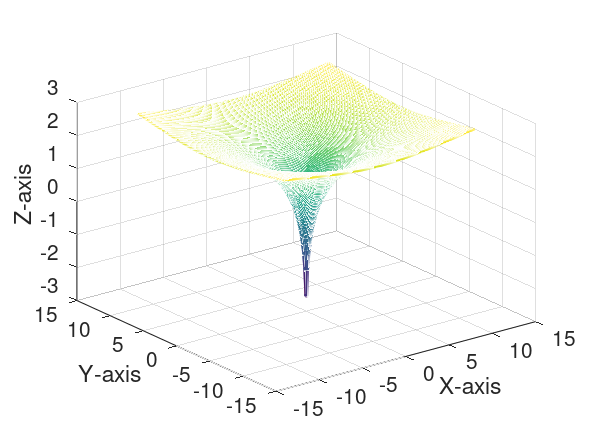
\includegraphics[scale=1.2]{Figure_2.png}
	\end{center}
	\caption{Streak Line and Path Line in an Unsteady Flow}
\end{figure}
\\Now to find streamline in this flow, we need to find velocity at each point. We can
find this by combined time streak markers. First we need to take snapshot of the flow
with combined time streak markers and a time t and t + $\delta$t . Connecting these markers gives an approximate direction of velocity at the point. The lines drawn connecting these dashes are the streamlines.
\begin{figure}[!ht]
	\begin{center}
			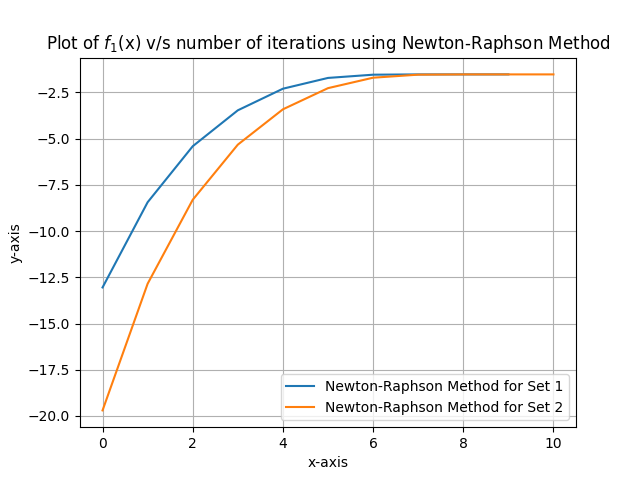
\includegraphics[scale=1.0]{Figure_3.png}
	\end{center}
	\caption{Stream Lines in an Unsteady Flow}
\end{figure}
\newpage
\noindent
The dotted streamline is one that passes through the point from which the
streak and path line emerge. We can see that the path line is not the same as streamline. If we compare the dotted streamline with the streak line entering through the same point, we can see that they aren’t same too. So in an unsteady flow, the steak line, path line and the time line aren’t the same and the velocity field is found by combined time streak markers.
\subsection{Terms relevant to Fluid Flow:}
The terms relevant to Fluid Flow across objects are described below:
\begin{itemize}
\item \textbf{Steady Flow}: A flow is said to be steady when the flow velocities and fluid properties at any point do not change with time. Flow in which any of these parameters change with time is said to be unsteady. A flow may appear steady or unsteady depending upon choice of coordinate axes.
\item \textbf{Uniform Flow}: A flow is said to be uniform when flow velocities and fluid properties do not change from point to point at any instant of time, or else the flow is non-uniform.
\item \textbf{Laminar Flow}: Type of fluid flow in which the fluid flows in infinitesimal parallel layers with no disruption between them. It is also referred to as streamline flow because it is characterized by non-crossing streamlines. For low values of Reynolds number, the flow is laminar.
\item \textbf{Turbulent Flow}: It is the type of fluid flow in which the fluid undergoes irregular fluctuations, or mixing. In this flow, the speed of a fluid particle at a point undergoes changes in both magnitude and direction continuously.
\item \textbf{Attached Flow}: It is the type of fluid flow where the fluid particles follow the boundary of the object’s surface. The flow stops at the surface as required by the no-slip boundary condition. 
\end{itemize}
\subsection{Terms relevant to Fluid Flow-lines:}
The terms relevant to Fluid Flow-lines are described below:
\begin{itemize}
\item \textbf{Path-lines}: Path-lines are the trajectories that individual fluid particles follow. These can be thought of as "recording" the path of a fluid element in the flow over a certain period. The direction the path takes will be determined by the streamlines of the fluid at each moment in time.
\item \textbf{Stream-lines}: A stream-line at any instant of time is an imaginary curve or line in the flow field so that the tangent to the curve at any point represents the direction of the instantaneous velocity at that point.
\item \textbf{Streak-lines}: A streak-line at any instant of time is the locus of the temporary locations of all fluid particles that have passed through a fixed point in the flow.
\end{itemize}
For a steady flow, the streamlines, path-lines and streak-lines are identical.
This is because in a steady flow, the properties at a point do not change with time.
Therefore, each particle on the stream-line will have the same velocity tangential to the stream-line curve and will follow the same path. This makes the path-line same as the stream-line.\\
\\Similarly, every fluid particle passing through a particular point will follow the same path as fluid properties are not changing with time. Therefore, at any instant of time, the streak-line will be the same as the stream-line.
\section{Experimental Apparatus:}
To visualize the flow across a body, the following apparatus is used:
\begin{itemize}
\item Smoke wind tunnel.
\item $CO_2$ tank.
\item Smoke generator (generates smoke by heating oil).
\item Objects to be tested.
\end{itemize}
The following figure shows a smoke wind tunnel.\\
The object we would like to test is fixed in the test section using a screw.\\
The smoke generator is turned on which causes the release of smoke into the test section through the 23 ports lining the base of the test section, each 7mm apart.\\
A $CO_2$ tank is used to release $CO_2$ that mixes with the smoke making the path-lines white and visible.\\
Above the test section is attached a pipe which carries the smoke out.\\
On the sides of the test section are attached lights that allow us to see the path of the smoke.\\
A fan is also present above the test section that maintains the desired wind velocity.
\begin{figure}[!ht]
	\begin{center}
			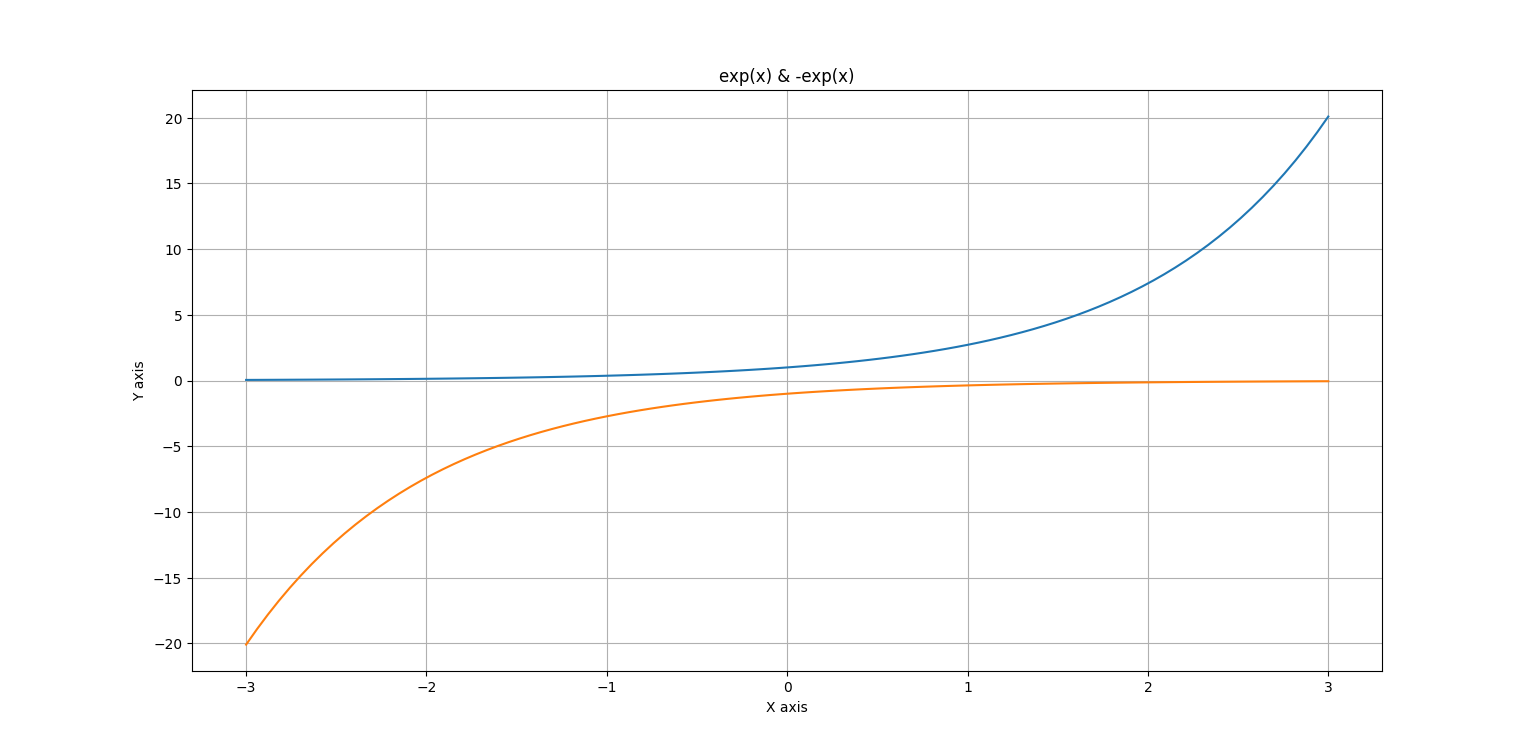
\includegraphics[scale=0.5]{Figure_1.png}
	\end{center}
	\caption{Smoke Wind Tunnel}
\end{figure}
\section{Experimental Procedure:}
To visualize the flow across a body, the following method is followed:
\begin{itemize}
\item Fix the object in the test-section.
\item Release the smoke.
\item Release the $CO_2$.
\item Observe the flow across the object.
\item Stop the smoke and $CO_2$ release.
\item Remove the object and place the next one.
\item Repeat the steps for an airfoil, a cylinder and a car model.
\end{itemize}
\section{Results:}
The following observations were made while performing this particular experiment:
\subsection{Airfoil When Angle of Attack = 0:}
The following figure shows the airflow across an airfoil when Angle of Attack = 0.\\
We can observe that the flow is attached initially.\\
In the central region, the flow is laminar and steady. The flow properties do not appear to change with time.\\
At the ends and above the airfoil, the flow is turbulent and unsteady. It is irregular and changes in space and time.\\
The flow is non-uniform and changes with location.
\begin{figure}[!ht]
	\begin{center}
			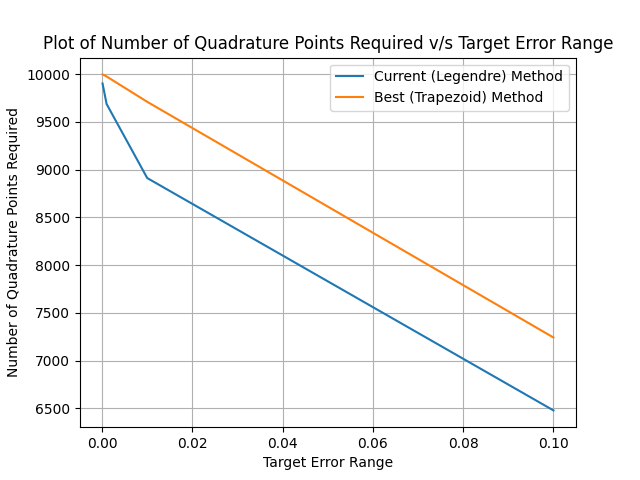
\includegraphics[scale=0.5]{Figure_4.png}
	\end{center}
	\caption{Flow across an Airfoil when Angle of Attack = 0}
\end{figure}
\newpage
\subsection{Airfoil When Angle of Attack $\neq$ 0:}
The following figure shows the airflow across an airfoil when Angle of Attack $\neq$ 0.\\
The air flows along a streamline (we can see the velocity of the smoke in the path-line tangential to the curve formed by the smoke) close to the underside of the airfoil.\\
The path-lines underside although bend, they retain their parallel nature, implying streamline motion.\\
The flow above the curved surface becomes highly turbulent after separating from the airfoil. A cloud of smoke forms which could be inferred as formation of vortices.
\begin{figure}[!ht]
	\begin{center}
			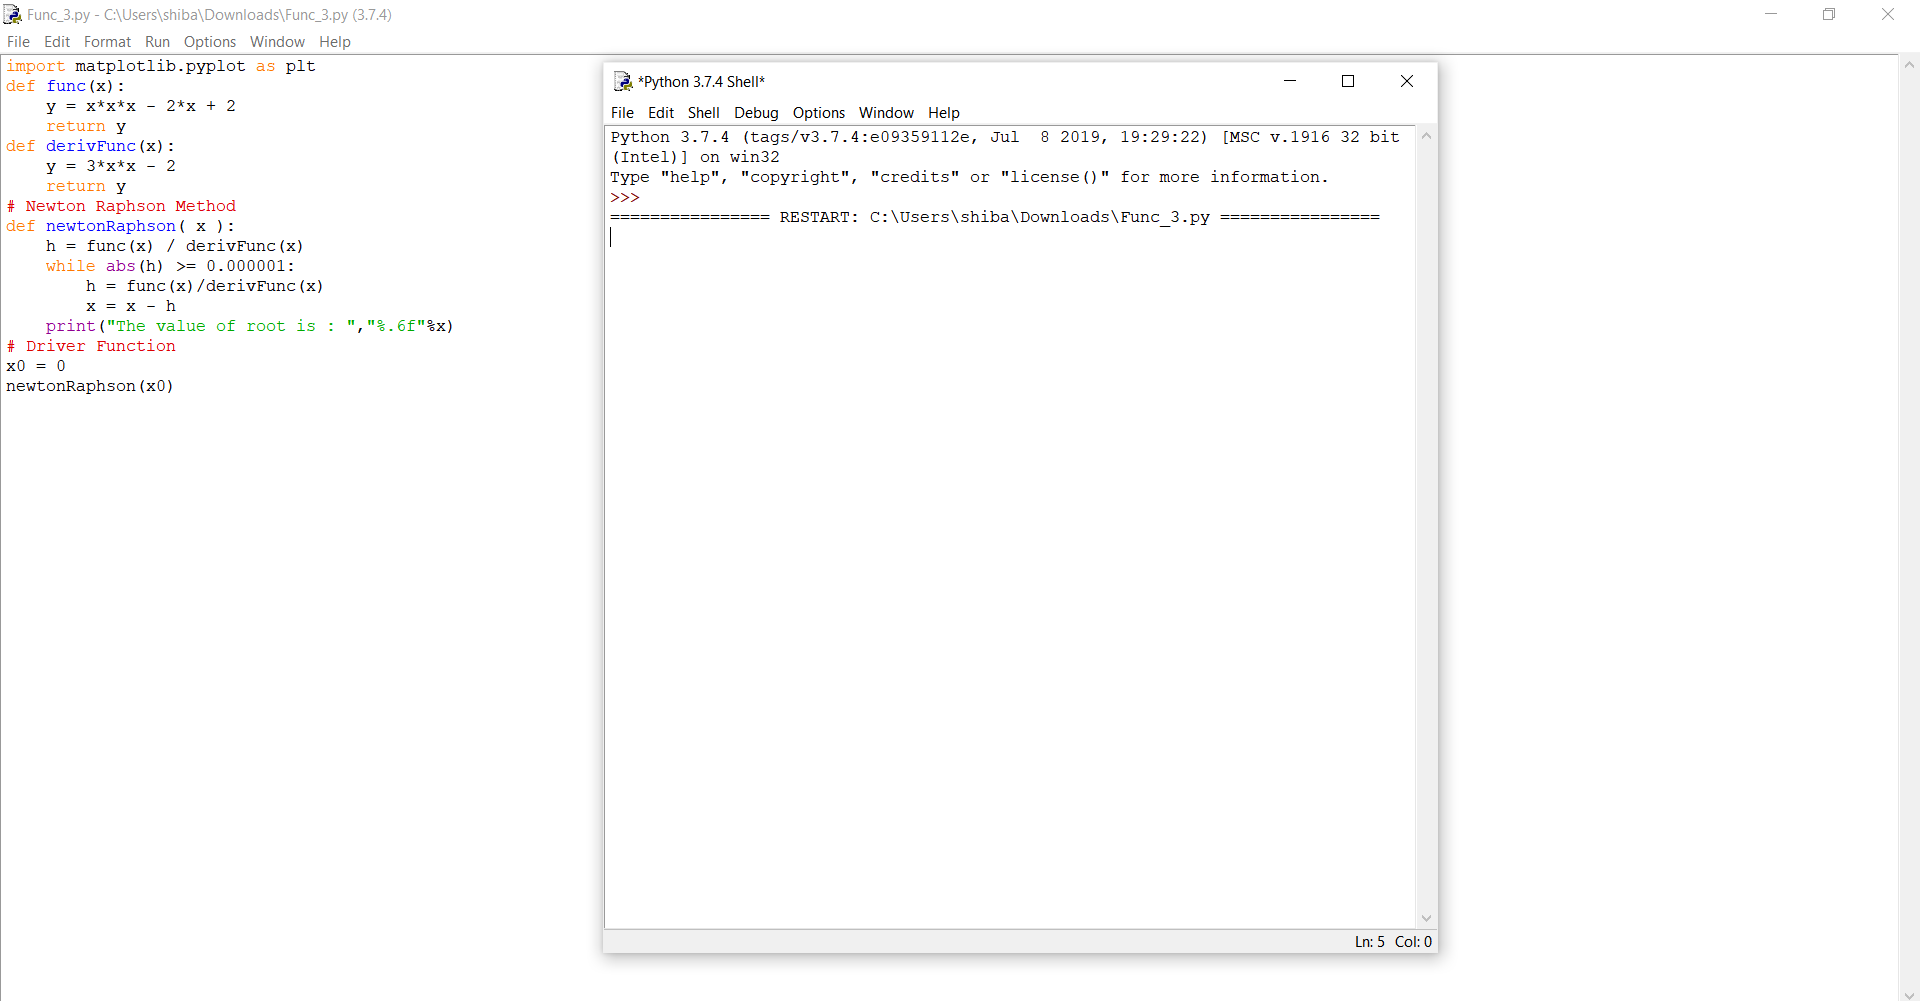
\includegraphics[scale=0.7]{Figure_11.png}
	\end{center}
	\caption{Flow across an Airfoil when Angle of Attack $\neq$ 0}
\end{figure}
\subsection{Cylinder:}
The following figure shows the airflow across a cylinder.\\
We can observe that the flow is attached initially.\\
In the central region, the flow is laminar and steady. The flow properties do not appear to change with time.\\
At the ends and above the airfoil, the flow is turbulent and unsteady. It is irregular and changes in space and time.\\
The flow is non-uniform and changes with location.
\newpage
\begin{figure}[!ht]
	\begin{center}
			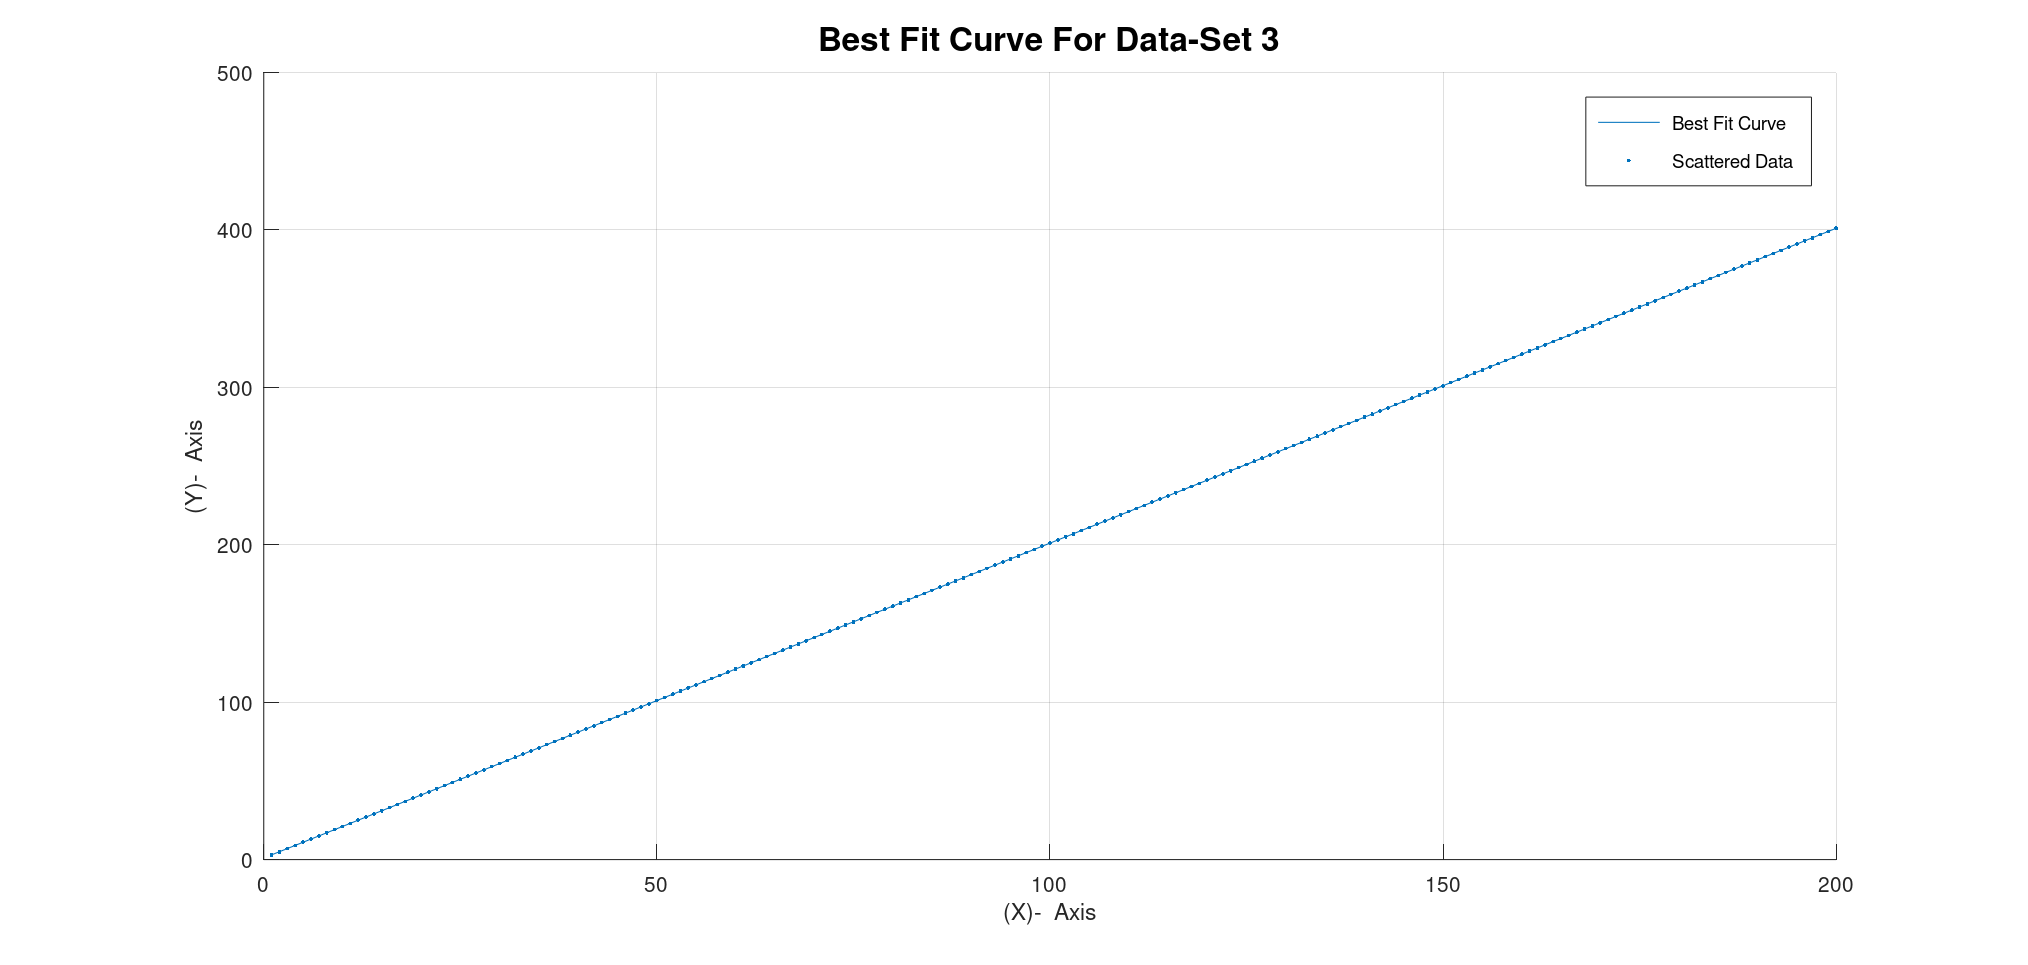
\includegraphics[scale=0.7]{Figure_5.png}
	\end{center}
	\caption{Flow across a Cylinder}
\end{figure}
\subsection{Car Model:}
The following figure shows the airflow across two different car models.\\
We can observe that the flow is attached initially. For these models it remains attached for much longer than the previous models.\\
The flow detaches later for the more slender car.\\
In the central region, the flow is laminar and steady. The flow properties here do not appear to change with time.\\
At the ends and above the airfoil, the flow is turbulent and unsteady. It is irregular and changes in space and time.\\
The flow is non-uniform and changes with location.\\
For the larger car, we observe a region of turbulent air flow behind it.
\newpage
\begin{figure}[h]
	\begin{center}
			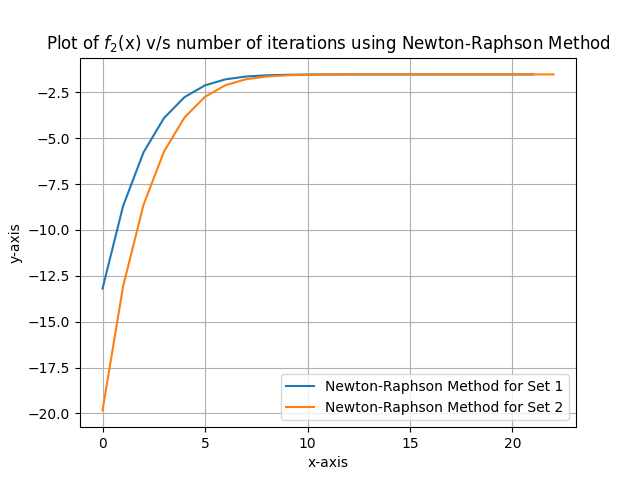
\includegraphics[scale=0.7]{Figure_6.png}
	\end{center}
	\caption{Flow across a Car Model}
\end{figure}
\section{Sources of Error:}
The following errors may occur while observing the airflow:
\begin{itemize}
\item Human error in observation.
\item Interference of external atmosphere with the airflow generated may make the airflow turbulent.
\end{itemize}
\section{Conclusion:}
Airflow across different objects varies with object geometry, nature of the flow set up and angle of attack among various parameters. This flow visualization technique gives us the means to observe the flow across objects and determine where the airflow gets detached. It is useful to make, modify and test our designs.
\end{document}
